\textbf{DAG}: Our compiler, FLAT, takes a DAG (Directed Acyclic Graph) as an input.
Every node in the DAG has input and output ports.
Nodes are either a primative operation such add addition or subtraction.
Or nodes are DAGs, allowing a nested structure. 

\textbf{IR}: After applying DAG transforms, FLAT transforms the DAG into a code like Internal Representation (IR).
It is easier to generate code from this IR than directly from the DAG.
Our IR comes in 2 flavours, loose and tight.
The loose IR is much more relaxed, using simple function signatures and allowing special types of temporary variables.
The tight IR is much stricter and closer to output code and requires the use of features such as complex function signatures.

\newsavebox{\looseIRlisting}
\begin{lrbox}{\looseIRlisting}% Store first listing
\minipage{.68\textwidth}
\begin{lstlisting}
define VOID @kernel (%in0, %in1) (%out0, %out1):
	%tmp1 = %in0
	%tmp2 = %tmp1 * %tmp1 * %tmp1
	%tmp3 = %in1
	%tmp4 = %tmp2 + %tmp3
	%tmp5 = %tmp4
	%tmp6 = %tmp2 - %tmp3
	%tmp7 = %tmp6
	%out0 = %tmp5
	%out1 = %tmp7
\end{lstlisting}
\endminipage
\end{lrbox}



\newsavebox{\tightIRlisting}
\begin{lrbox}{\tightIRlisting}% Store first listing
\minipage{.68\textwidth}
\begin{lstlisting}
define VOID @kernel (new #list(in), new #list(out)):
	new #tmp2 = #in[0] * #in[0] * #in[0]
	#out[0] = #tmp2 + #in[1]
	#out[1] = #tmp2 - #in[1]
	<return nothing>
\end{lstlisting}
\endminipage
\end{lrbox}

\begin{figure}
\centering

\sbox{\measurebox}{%
  \begin{minipage}{.68\textwidth} \centering
        \subfloat[Loose IR]{\label{fig:figB}\usebox{\looseIRlisting}}
        \vspace{1em}
        \subfloat[Tight IR]{\label{fig:figC}\usebox{\tightIRlisting}}
  \end{minipage}
}

\usebox{\measurebox}\qquad
    \begin{minipage}[][\ht\measurebox][c]{.26\textwidth}
      \subfloat[Input DAG]{\label{fig:loose_tight_dag}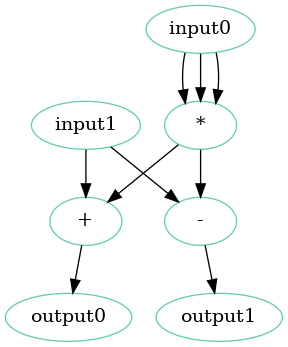
\includegraphics[width=\textwidth]{tight_vs_loose.png}}
       
    \end{minipage}
\caption{Example of the difference between a loose IR and tight IR. Figure \ref{fig:loose_tight_dag} shows the corresponding input DAG.} 
\label{fig:tight_loose}
\end{figure}

    \begin{figure}[h!]
    \begin{center}
        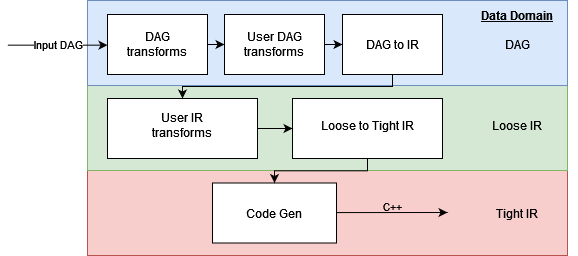
\includegraphics[width=.7
        \textwidth]{comp-arch.png}
        \caption{Overview of FLAT's architecture.}
        \label{fig:arch}
    \end{center}
\end{figure}